\documentclass{beamer}
\usetheme{metropolis}
\usepackage{graphicx}
\usepackage{amsmath}
\usepackage{tcolorbox}
\title{Elementary Statistics: Math 080}
\author{Jordan Hanson}
\institute{Whittier College Department of Physics and Astronomy}

\begin{document}
\maketitle

\section{Summary}

\begin{frame}{Summary}
Unit 2 and 3
\begin{enumerate}
\item Central Limit Theorem: 7.1
\item Confidence Intervals and Hypothesis Testing
\begin{itemize}
\item Confidence intervals and data interpretation: 8.1 - 8.4
\item Rejecting the null hypothesis, types of error, underlying distributions: 9.1 - 9.3, 9.6
\end{itemize}
\end{enumerate}
\end{frame}

\section{The Central Limit Theorem}

\begin{frame}{The Central Limit Theorem}
\begin{tcolorbox}[colback=orange!10,colframe=orange!100,title=The Central Limit Theorem]
\textbf{Central Limit Theorem:} Let X be a continuous random variable, with mean $\mu_x$ and standard deviation $\sigma_x$.  The average $\bar{x}$ of $n$ values of X is normally distributed like $N(\mu_x,\sigma_x/\sqrt{n})$.
\end{tcolorbox}
\end{frame}

\begin{frame}{The Central Limit Theorem}
\begin{figure}
\centering
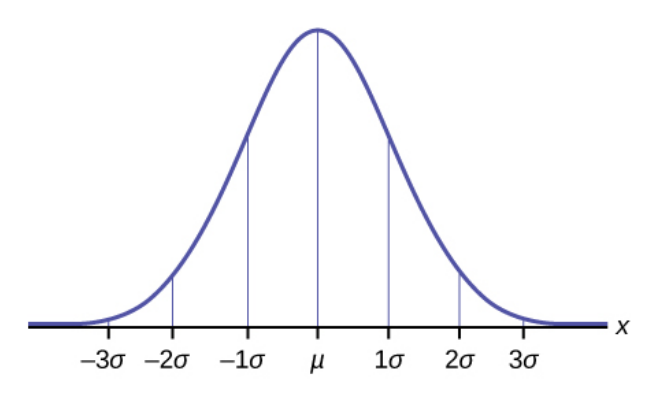
\includegraphics[width=0.5\textwidth]{figures/norm.png}
\caption{\label{fig:norm} The normal distribution about a mean $\mu$ with the units of standard deviations shown.}
\end{figure}
\textbf{Example:} An unknown distribution has a mean of $\mu = 90$ and a standard deviation of $\sigma = 15$. Samples of size $n = 25$ are drawn randomly from the population.  Find the probability that the \textit{sample mean} is between 87 and 93. \\ \vspace{1cm}
\end{frame}

\section{Interactive Questions}

\begin{frame}{Interactive Questions: Central Limit Theorem}
Suppose we take samples of size $n = 16$ from a large data set and compute the averages and standard deviations of the samples.  Suppose we repeat the whole process, but change $n = 100$.  Which of the following is true?
\begin{itemize}
\item A: The means of our samples will shift upwards by a factor of $100/16$.
\item B: The means of our samples will shift downwards by a factor of $100/16$.
\item C: The standard deviations of our samples will shift downwards by a factor of $\sqrt{100/16}$.
\item D: The standard deviations of our samples will shift upwards by a factor of $\sqrt{100/16}$.
\end{itemize}
\end{frame}

\begin{frame}{Interactive Questions: Central Limit Theorem}
Suppose we take samples of size $n = 100$ from a large data set that has mean $\mu$ and standard deviation $\sigma$, and compute the averages and standard deviations of the \textit{samples}.  Which of the following is true?
\begin{itemize}
\item A: Each standard deviation of each sample we collect will be $\sigma/10$.
\item B: The standard deviation of the means of our samples will be $\sigma/10$.
\item C: Each mean of each sample we collect will be $\mu/10$.
\item D: The mean of the means of our samples will be $\mu$.
\end{itemize}
\end{frame}

\end{document}